% !TeX program = lualatex

\documentclass[12pt]{article}



\usepackage[margin=1in]{geometry} 
\usepackage{amsmath,amsthm,amssymb}
\usepackage{MnSymbol}
\usepackage{graphicx}
\usepackage{bm}
\usepackage[normalem,normalbf]{ulem}
\usepackage{algorithm} 
\usepackage{algpseudocode} 
\usepackage{multirow}
\usepackage{rotating}
\usepackage{therefore}

\usepackage{tikz}
\usetikzlibrary{shapes.multipart}
\usetikzlibrary{shapes.symbols}

\usetikzlibrary{graphs,graphdrawing,graphs.standard,quotes}
\usegdlibrary{circular,force,layered,routing}
\tikzset{
	graphs/simpleer/.style={
		nodes={draw,circle, blue, left color=blue!20, text=black, inner sep=1pt},
		node distance=2.5cm, nodes={minimum size=2em}
	},
	every loop/.style={},
}

\newcommand*\circled[1]{\tikz[baseline=(char.base)]{
		\node[shape=circle,draw,inner sep=2pt] (char) {#1};}}

\newcommand{\m}{\medskip\\}
\newcommand{\N}{\mathbb{N}}
\newcommand{\Z}{\mathbb{Z}}
\newcommand{\R}{\mathbb{R}}
\newcommand{\bbs}{\textbackslash\textbackslash\space}
\newcommand{\bs}{\textbackslash\space}
\newcommand{\la}{\enskip\land\enskip}
\newcommand{\lo}{\enskip\lor\enskip}
\newcommand{\comp}[1]{#1^\mathsf{c}}
\newcommand{\micdrop}{\qed}
\newcommand{\contra}{\begin{tikzpicture}
		\node[starburst, draw, minimum width=3cm, minimum height=2cm,line width=1.5pt,red,fill=yellow,scale=.5]
		{BOOM, A CONTRADICTION!!!};
\end{tikzpicture}}

\renewcommand{\qedsymbol}{$\blacksquare$}

\DeclareMathOperator{\lcm}{lcm}

\newtheorem{theorem}{Theorem}

\newenvironment{exercise}[2][Exercise]{\begin{trivlist}
		\item[\hskip \labelsep {\bfseries #1}\hskip \labelsep {\bfseries #2.}]}{\end{trivlist}}

\setlength\parindent{24pt}

\makeatletter
\renewcommand*\env@matrix[1][*\c@MaxMatrixCols c]{%
	\hskip -\arraycolsep
	\let\@ifnextchar\new@ifnextchar
	\array{#1}}
\makeatother
\setlength\parindent{24pt}


\begin{document}
	
	% --------------------------------------------------------------
	%                         Start here
	% --------------------------------------------------------------
	
	
	\title{Homework 9 (Due March 28, 2023)}
	\author{Jack Hyatt\\ %replace with your name
		MATH 575 - Discrete Mathematics II - Spring 2023} 
	
	\maketitle
	
	Justify all of your answers completely.\m
	Collaborators: Chance and Nathan. Anyone else that claimed I helped is just plain wrong.
	
	
	\medskip 
	
	\begin{enumerate}

\item Recall that $Q_d$ is the $d$-dimensional hypercube. For every $d \geq 1$, give an explicit edge-coloring to prove $\chi'(Q_d) = \Delta(Q_d)$. 
\begin{proof}
	Every vertex in a $d$-dimensional hypercube will have $d$ neighbors, since there are $d$ bits in the corresponding bitstring.\\
	Let us create a coloring by looking at a vertex. Since there will be an edge to another vertex iff a single bit in the bitstrings differ, the edge created is not adjacent to any other edge that exists from same bit differing. So let us color the edge color $i$, where $i$ is the index of the differing bit. This gives us $d$ colors for a vertex, and each color will never be adjacent to the same color.
\end{proof}
\medskip 

\item Recall that $\alpha'(G)$ denotes the size of a maximum matching in $G$.
\begin{enumerate}
\item Prove that $\chi'(G) \geq \frac{|E(G)|}{\alpha'(G)}$. 
\begin{proof}
	Considering a proper edge coloring, the color classes partition the graph into disjoint matchings. The minimum number of color classes would be in the case where every color class had the size of the biggest matching, since the classes are disjoint matchings themselves. So that case is $\frac{|E(G)|}{\alpha'(G)}$, which is the minimum case. \Therefore $\chi'(G) \geq \frac{|E(G)|}{\alpha'(G)}$. 
\end{proof}
\item Prove that if $G$ is a $k$-regular graph with no perfect matching, then $\chi'(G) =\Delta(G)+1$. 	
\begin{proof}
	BWOC, assume $\chi'(G) \neq \Delta(G)+1$ and $G$ is $k$-regular with no perfect matching. By Vizing's theorem, we can then assume $\chi'(G) = \Delta(G) = k$.\\
	We also know that $\chi'(G)\geq\frac{|E(G)|}{\alpha'(G)}$. We'll then get $k \geq \frac{kn}{2\alpha'(G)} \implies \alpha'(G)\geq \frac{n}{2} \implies$ there exists a perfect matching, \contra
	
\end{proof}
\end{enumerate}


\medskip

\item Chromatic number versus edge-chromatic number
\begin{enumerate}
\item  For every $n \geq 4$, construct a graph $G$ on $n$-vertices with $\chi(G) < \chi'(G)$.\m
$K_{1,n-1}$. It is bipartite, so $\chi(G) =2$, but also $\chi'(G)$ will be the degree of the lone vertex in the smaller bipartition, which will be at least 3 since $n\geq4$.
\item Give a characterization of all connected graphs for which $\chi(G) > \chi'(G)$. That is, prove a statement of the form:

``If $G$ is a connected graph, then $\chi(G) > \chi'(G)$ if and only if $\makebox[2cm]{\hrulefill}$."\m
The claim I will make is $\chi(G) > \chi'(G)$ if and only if $G$ is $K_{2m}$.
\begin{proof}
	($\Longrightarrow$)\\
	Assume $\chi(G) > \chi'(G)$. Then by Vizing's theorem, we get $\chi(G) > \Delta(G)$. Then by Brooks' theorem, will get that $G$ is an odd cycle or a complete graph. We know it isn't an odd cycle since $\chi'(C_{2n+1}) = 3 = \chi(C_{2n+1})$. So it must be a complete graph.\\
	We also know from class that $\chi'(K_{2m}) = \Delta(K_{2m})$ and $\chi'(K_{2m+1}) = \Delta(K_{2m+1})+1$. Then because of that and $\Delta(G)+1 \geq \chi(G) > \chi'(G)$, $G$ must be $K_{2m}$.\\
	($\Longleftarrow$)\\
	Assume $G$ is $K_{2m}$. Then $\chi(G)= 2m = \Delta(G)+1$ since every node is adjacent to every other node. We also know from class that $\chi'(G) = \Delta(G) = 2m-1$. So $\chi(G) > \chi'(G)$.
\end{proof}
\end{enumerate}
\medskip

\item Determine for which values $d$ the hypercube $Q_d$ is planar and for which values it is non-planar.\m
$Q_1$ and $Q_2$ are trivially planar. Below is $Q_3$.
\begin{center}
	\tikz \graph [nodes={draw, circle}, clockwise, phase=45] {
		subgraph C_n [V={000,001,010,011}, radius=2.5cm] -- subgraph C_n [V={100,101,110,111}, radius=0cm]
	};
\end{center}
$Q_4$ is not planar since it has $\frac{dn}{2} = 32$ edges, and we showed in class any planar graph will satisfy the inequality $e\leq2n-4$, which $Q_4$ does not $(32\geq 28)$. By extension, any $Q_{\geq4}$ is not planar since it would contain a copy of $Q_4$.

\medskip 
\item Use Euler's Formula to prove that the Petersen graph (drawn below) is not planar.
{\em Do not use Wagner's Theorem or Kuratowski's Theorem.}
\begin{center}
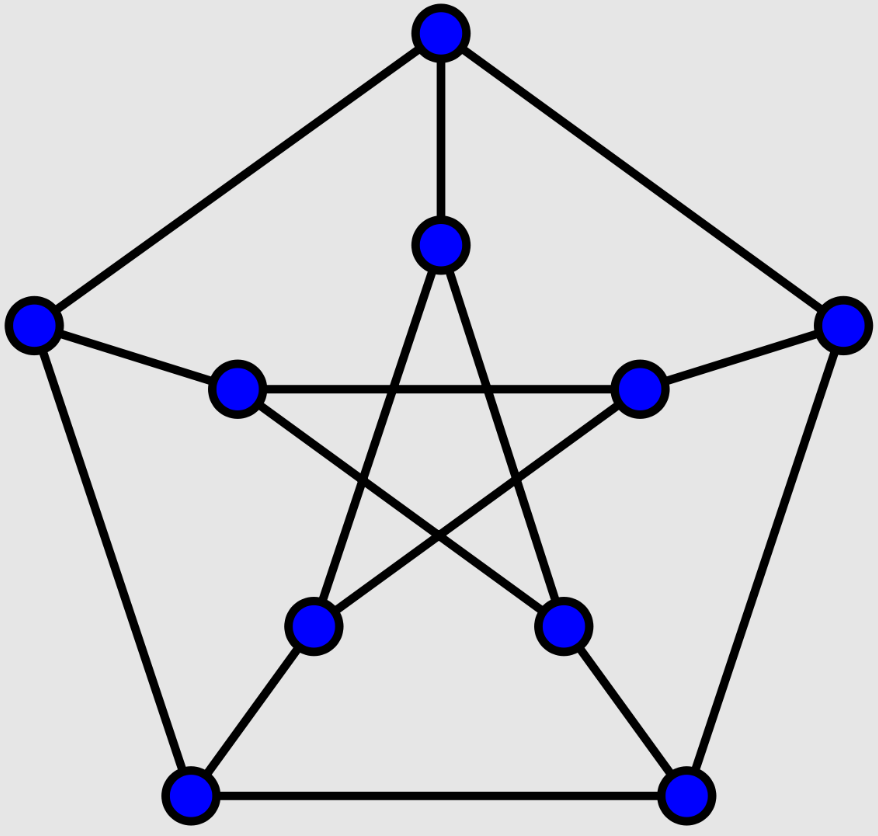
\includegraphics[scale=.1]{petersen.png}
\end{center}
\begin{proof}
	BWOC, assume Euler's Formula holds true.\\
	The graph has 10 vertices and 15 edges, so the number of faces must be 7. We also have that there are no cycles of length 3 or 4. So then with degree sum formula, we get that \[2e = \sum_{f'\text{ in faces}} \ell(f') \geq 5f \implies f \leq 6\]
	which is\contra
\end{proof}
\end{enumerate}

\end{document}
